\chapter{有机分子：骨架与命名}\label{ch:g11:organic-skeletons}

一次性打火机里装的是丁烷，它在压强下呈液态；登上雪山的野营炉气罐里装的是丙烷，
或是丙烷含量更高的混合气。两者都只由碳原子和氢原子构成，
并且同属一个庞大的家族：以碳原子为骨架构建的分子。
这类分子已知的多达数百万种。要谈论它们，
化学家需要既能快速画出它们，
又能无歧义地为它们命名的方法。

\begin{recall}
碳形成四个共价键，氢形成一个共价键；在与四个单键相连的碳原子周围，
这些键指向正四面体的顶点，
键角约为 \ang{109.5}（见\cref{ch:g10:lewis-and-shape}）。
\end{recall}

\begin{omfigure}
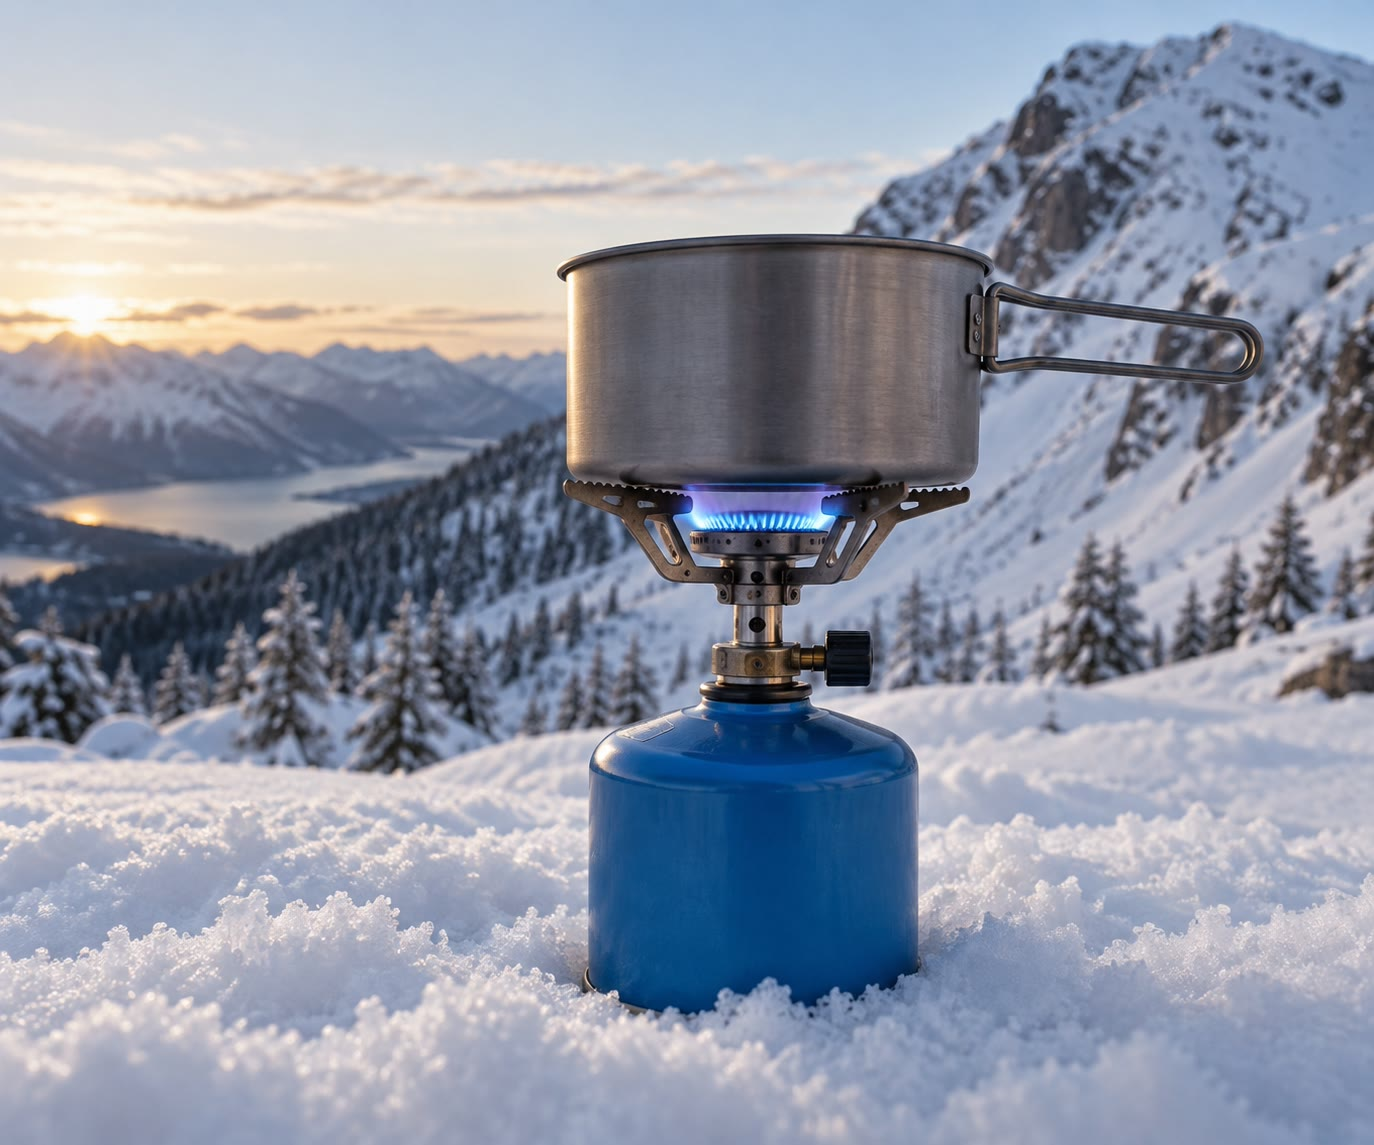
\includegraphics[width=0.48\linewidth]{images/book1/ai/g11-camping-cartridge.jpg}

{\small 雪地中的野营炉，正在燃烧
由碳和氢构成的气体。}
\end{omfigure}

\section{有机分子的化学式}

\begin{definition}[有机化合物]\label{def:g11:organic-skeletons:organic}
称\emph{有机化合物}\index{有机化合物}为分子以碳原子为骨架构建的化合物，
这些碳原子彼此相连，并与氢原子相连，
骨架上还可能连有氧、氮等其他原子。
（二氧化碳、一氧化碳和碳酸盐，
传统上不计入有机化合物。）
\end{definition}

\begin{definition}[四种化学式]\label{def:g11:organic-skeletons:formulas}
分子可以用四种方式表示：
\begin{itemize}
  \item 其\emph{分子式}\index{分子式}
        只给出每种元素的原子个数，例如 \ce{C4H10}；
  \item 其\emph{结构式}\index{结构式}
        显示每一个原子和每一个化学键；
  \item 其\emph{结构简式}\index{结构简式}
        显示碳原子之间的化学键，并把氢原子
        与其所连的碳原子归为一组，例如 \ce{CH3-CH2-CH2-CH3}；
  \item 其\emph{键线式}\index{键线式}
        只用折线画出碳骨架的化学键：每个端点和每个拐点
        都是一个碳原子，与碳相连的氢原子不画出，
        其他原子（连同其所连的氢原子）则要写出。
\end{itemize}
\end{definition}

\begin{omfigure}
\setchemfig{atom sep=1.45em}
\renewcommand{\arraystretch}{1.6}
\small
\begin{tabular}{@{}l@{\quad}c@{\quad}c@{}}
 & 丁烷 & 2-甲基丙烷 \\
分子式 & \ce{C4H10} & \ce{C4H10} \\[4pt]
结构式 &
\chemfig{H-C(-[2]H)(-[6]H)-C(-[2]H)(-[6]H)-C(-[2]H)(-[6]H)-C(-[2]H)(-[6]H)-H} &
\chemfig{H-C(-[2]H)(-[6]H)-C(-[6]H)(-[2,1.5]C(-[1]H)(-[3]H)(-[2]H))-C(-[2]H)(-[6]H)-H} \\[10pt]
结构简式 & \ce{CH3-CH2-CH2-CH3} &
\chemfig{CH_3-CH(-[6]CH_3)-CH_3} \\[14pt]
键线式 & \chemfig{-[:30]-[:-30]-[:30]} & \chemfig{-[:30](-[:90])-[:-30]} \\
\end{tabular}

{\small 丁烷和 2-甲基丙烷的四种化学式。在键线式中，
线段的每个端点和每个拐点都是一个碳原子：
各含四个碳原子。}
\end{omfigure}


\begin{example}[读懂键线式]\label{ex:g11:organic-skeletons:reading}
在丁烷的键线式中，折线有两个端点和两个拐点，共四个碳原子。
端点碳原子只画出一个化学键，因此连有三个氢原子（\ce{CH3}）；
拐点碳原子画出两个化学键，因此连有两个氢原子（\ce{CH2}）。
每个碳原子共有四个化学键，
由此得到 \ce{C4H10}。
\end{example}

\section{碳链}

分子的碳骨架可以是\emph{直链}，即每个碳原子至多与另外两个碳原子相连，
如丁烷；也可以是\emph{支链}，即至少有一个碳原子与另外三个或四个碳原子相连，
如 2-甲基丙烷；还可以是\emph{环}，如环己烷 \ce{C6H12}，
其键线式为一个六边形。
链状结构用折线表示，是因为每个碳原子周围的实际化学键夹角约为 \ang{109.5}，
而非 \ang{180}：
所谓“直链”，实际上是空间中的折线。

\begin{omfigure}
\setchemfig{atom sep=1.9em}
\begin{tabular}{ccc}
\chemfig{-[:30]-[:-30]-[:30]-[:-30]-[:30]} &
\chemfig{-[:30](-[:90])-[:-30]-[:30](-[:90])-[:-30]} &
\chemfig{*6(------)} \\[4pt]
\small 直链：己烷 & \small 支链：2,4-二甲基戊烷 &
\small 环：环己烷 \\
\small \ce{C6H14} & \small \ce{C7H16} & \small \ce{C6H12}
\end{tabular}

{\small 三种碳骨架，用键线式表示。}
\end{omfigure}

\section{烷烃及其命名}

\begin{definition}[烷烃，烷基]\label{def:g11:organic-skeletons:alkane}
称\emph{烷烃}\index{烷烃}为仅由碳和氢组成的化合物，
其骨架为链状（直链或支链，不是环），且只含单键；
其分子式为 \ce{C_{n}H_{2n+2}}。称\emph{烷基}\index{烷基}
为烷烃去掉一个氢原子后剩下的基团，
它可以与链相连：甲基
\ce{-CH3}、乙基 \ce{-CH2-CH3}。
\end{definition}

\begin{omfigure}
\begin{tabular}{rlcrlc}
\hline
$n$ & 名称 & 分子式 & $n$ & 名称 & 分子式 \\
\hline
1 & 甲烷 & \ce{CH4}    & 6  & 己烷 & \ce{C6H14} \\
2 & 乙烷  & \ce{C2H6}   & 7  & 庚烷 & \ce{C7H16} \\
3 & 丙烷 & \ce{C3H8}   & 8  & 辛烷 & \ce{C8H18} \\
4 & 丁烷  & \ce{C4H10}  & 9  & 壬烷 & \ce{C9H20} \\
5 & 戊烷 & \ce{C5H12}  & 10 & 癸烷 & \ce{C10H22} \\
\hline
\end{tabular}\par\medskip

{\small 前十种直链烷烃。含 $n$ 个碳原子的链，
其名称为相同词根加\emph{-ane}；烷基则
把\emph{-ane}换成\emph{-yl}（甲基、乙基、丙基……）。}
\end{omfigure}

\begin{method}[烷烃的命名]\label{met:g11:organic-skeletons:naming}
\begin{enumerate}
  \item 找出最长的碳链，它给出词根名称
        （如戊烷、己烷……）。
  \item 不在主链上的原子构成与之相连的烷基，
        即取代基。
  \item 从能使取代基位次最小的一端
        给主链编号。
  \item 将每个取代基连同其位次（在链上的位置）
        按字母顺序写在词根之前；相同基团
        用词头二、三、四表示，每个基团各标一个位次。
        位次之间用逗号分隔，数字与文字之间用连字符连接。
\end{enumerate}
\end{method}

\begin{omfigure}
\begin{tikzpicture}[font=\small, x=0.9cm, y=0.9cm]
  % main chain of 5, zigzag; methyls on C2 and C3
  \coordinate (a1) at (0,0); \coordinate (a2) at (0.87,0.5);
  \coordinate (a3) at (1.73,0); \coordinate (a4) at (2.6,0.5);
  \coordinate (a5) at (3.46,0);
  \coordinate (m2) at (0.87,1.5); \coordinate (m3) at (1.73,-1);
  \draw[line width=1pt] (a1) -- (a2) -- (a3) -- (a4) -- (a5);
  \draw[line width=1pt] (a2) -- (m2); \draw[line width=1pt] (a3) -- (m3);
  \foreach \k in {1,2,3,4,5}
    \node[omDef, font=\footnotesize\bfseries, fill=white, inner sep=1pt]
      at ($(a\k)+(0,-0.32)$) {\k};
  \draw[omProp, thick] (m2) circle (0.28);
  \draw[omProp, thick] (m3) circle (0.28);
  \node[omProp, anchor=west] at ($(m2)+(0.35,0)$) {C2 上的甲基};
  \node[omProp, anchor=west] at ($(m3)+(0.35,0)$) {C3 上的甲基};
  \node[anchor=west, align=left] at (5,0.3) {最长链：5 个碳，
    \emph{戊烷}\\ 从左编号：2 和 3\\ （从右编号：3
    和 4，较大）\\ 名称：\textbf{2,3-二甲基戊烷}};
\end{tikzpicture}

{\small 支链烷烃的命名：主链（已编号）、
取代基（圈出）和名称。}
\end{omfigure}

\begin{method}[由名称写出键线式]\label{met:g11:organic-skeletons:drawing}
\begin{enumerate}
  \item 画出由词根给出的主链，画成锯齿形，
        并给其碳原子编号。
  \item 在各取代基对应的位次上连接该取代基。
  \item 检查：数出碳原子数，并检查
        每个碳原子的键数不超过四个。
\end{enumerate}
\end{method}

\section{同分异构体}

\begin{definition}[同分异构体，构造异构体]\label{def:g11:organic-skeletons:isomer}
称\emph{同分异构体}\index{同分异构体}为分子式相同的
不同化合物。称\emph{构造异构体}\index{构造异构体}为
原子之间成键顺序不同的同分异构体，
例如碳骨架不同。
\end{definition}

\begin{proposition}[同分异构体具有不同的性质]\label{prop:g11:organic-skeletons:properties}
% ledger: bp:C4H10, bp:isobutane, bp:C5H12, bp:isopentane, bp:neopentane
构造异构体是不同的物质，具有不同的性质。
在给定分子式的烷烃同分异构体中，支链越多，
沸点越低：丁烷的沸点约为 \qty{0}{\celsius}，
2-甲基丙烷为 \qty{-11.7}{\celsius}；戊烷为
\qty{36.1}{\celsius}，2-甲基丁烷为 \qty{27.8}{\celsius}，
2,2-二甲基丙烷为 \qty{9.5}{\celsius}。
\end{proposition}

\begin{proof}
这些数值是测量得到的。支链分子更紧凑，
与邻近分子接触的表面较少，其范德瓦耳斯
相互作用较弱（见\cref{ch:g11:polarity-and-cohesion}）。
\end{proof}

\begin{omfigure}
\setchemfig{atom sep=2em}
\begin{tabular}{ccc}
\chemfig{-[:30]-[:-30]-[:30]-[:-30]} &
\chemfig{-[:30](-[:90])-[:-30]-[:30]} &
\chemfig{-[:0](-[:90])(-[:-90])-[:0]} \\[24pt]
\small 戊烷 & \small 2-甲基丁烷 & \small 2,2-二甲基丙烷 \\
\small \qty{36.1}{\celsius} & \small \qty{27.8}{\celsius} &
\small \qty{9.5}{\celsius}
\end{tabular}
\medskip

{\small \ce{C5H12} 的三种同分异构体及其沸点：
支链越多，沸点越低。}
\end{omfigure}

\section{原油中的烷烃}

原油是由数千种化合物组成的混合物，其中大多数为烷烃，
碳原子数从 1 个到 40 多个不等。在炼油厂中，原油被加热，其蒸气沿一根高塔上升，
越往塔顶温度越低：
每一馏分在温度与其沸程相符的高度处凝结。
气体（甲烷至丁烷）从塔顶逸出，随后是汽油、
煤油、柴油；重质油和沥青则留在塔底。此即
分馏，依沸点高低加以分离，对烷烃而言，沸点
随碳链加长而升高。

\begin{omfigure}
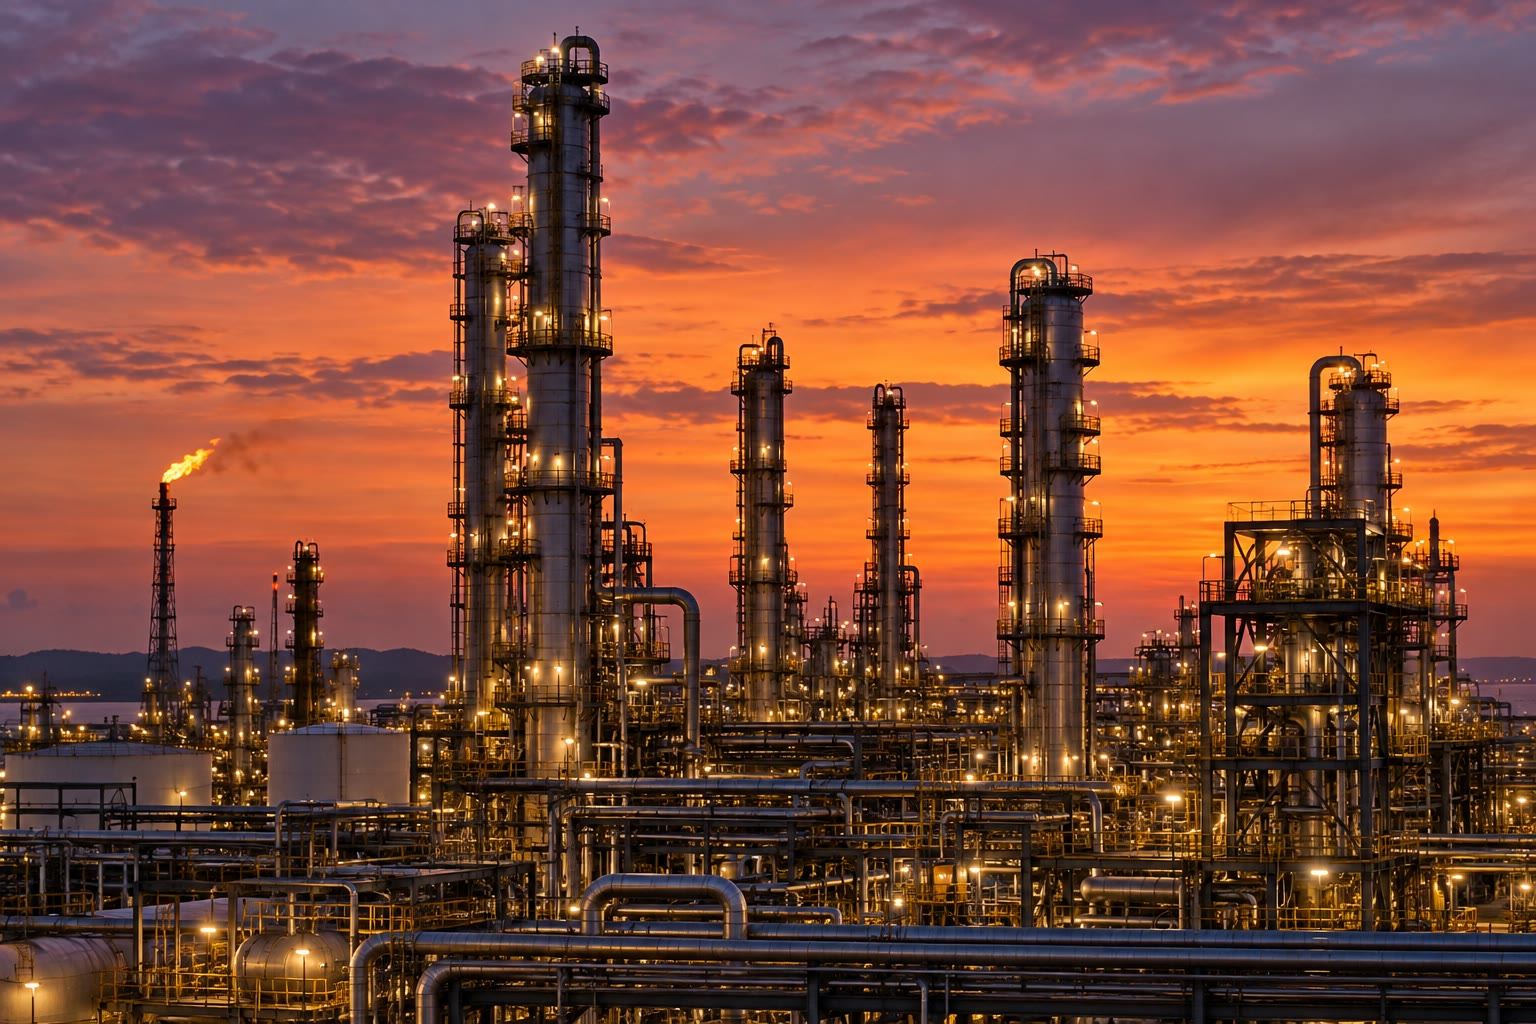
\includegraphics[width=0.52\linewidth]{images/book1/ai/g11-refinery-dusk.jpg}

{\small 黄昏时的炼油厂分馏塔。}
\end{omfigure}

\begin{safety}{\ghs[0.66cm]{GHS02}\ghs[0.66cm]{GHS04}\ghs[0.66cm]{GHS07}\ghs[0.66cm]{GHS08}\ghs[0.66cm]{GHS09}}
% ledger: ghs:butane, ghs:pentane
丁烷是一种极易燃的气体，须加压储存。戊烷是
一种高度易燃的液体；其蒸气会引起嗜睡，若吞食可能损伤
肺部，且对水生生物有毒。勿使明火靠近
轻质烷烃；应在通风橱中操作。
\end{safety}

\section{练习}


\begin{exercise}[$\star$]\label{exo:g11:organic-skeletons:1}
写出此处所画分子的分子式，并判断它们是否为
同分异构体：
\setchemfig{atom sep=1.6em}
\chemfig{-[:30]-[:-30]-[:30]-[:-30]-[:30]} \quad 和 \quad
\chemfig{-[:30](-[:90])-[:-30]-[:30]-[:-30]}.
\end{exercise}

\begin{exercise}[$\star$]\label{exo:g11:organic-skeletons:2}
命名：\ce{CH3-CH2-CH3}；\ce{CH3-CH2-CH2-CH2-CH2-CH3}；
\chemfig{CH_3-CH(-[2]CH_3)-CH_2-CH_3}.
\end{exercise}

\begin{exercise}[$\star$]\label{exo:g11:organic-skeletons:3}
写出丙烷和 2-甲基丙烷的结构简式，以及
乙烷的结构式。
\end{exercise}

\begin{exercise}[$\star$]\label{exo:g11:organic-skeletons:4}
数出每个分子中的碳原子和氢原子个数：
\setchemfig{atom sep=1.6em}
\chemfig{-[:30]-[:-30](-[:-90])-[:30]-[:-30]} \quad 和 \quad
\chemfig{*6(------)}.
\end{exercise}

\begin{exercise}[$\star$]\label{exo:g11:organic-skeletons:5}
写出碳原子数为 8 的烷烃的分子式，并求氢原子数为 20 的
烷烃所含的碳原子数。
\end{exercise}

\begin{exercise}[$\star\star$]\label{exo:g11:organic-skeletons:6}
画出 3-甲基己烷、2,2-二甲基丁烷和
3-乙基戊烷的键线式，并写出它们的分子式。
\end{exercise}

\begin{exercise}[$\star\star$]\label{exo:g11:organic-skeletons:7}
画出并命名 \ce{C5H12} 的三种同分异构体。
\end{exercise}

\begin{exercise}[$\star\star$]\label{exo:g11:organic-skeletons:8}
下列名称均有误。画出每个分子，并给出其正确名称：
2-乙基丁烷；4-甲基戊烷；1-甲基丁烷。
\end{exercise}

\begin{exercise}[$\star\star$]\label{exo:g11:organic-skeletons:9}
利用 \ce{C5H12} 同分异构体的图，按沸点对它们排序，
并解释这一顺序。
\end{exercise}

\begin{exercise}[$\star\star$]\label{exo:g11:organic-skeletons:10}
环己烷为 \ce{C6H12}，己烷为 \ce{C6H14}。试解释为何少了两个氢原子，
并判断这两种化合物是否互为同分异构体。环己烷是否属于
烷烃？
\end{exercise}

\begin{exercise}[$\star\star$]\label{exo:g11:organic-skeletons:11}
在丙烷、丁烷、2-甲基丙烷和环丁烷（\ce{C4H8}，
由四个碳原子构成的环）中，哪些彼此互为同分异构体？
\end{exercise}

\begin{exercise}[$\star\star\star$]\label{exo:g11:organic-skeletons:12}
画出并命名 \ce{C6H14} 的五种同分异构体。
\end{exercise}

\begin{exercise}[$\star\star\star$]\label{exo:g11:organic-skeletons:13}
想象直链烷烃像一条长长的锯齿，支链很多的烷烃则像一个
小球。借助这一图像，解释支链增多为何会降低同分异构体的
沸点。
\end{exercise}

\begin{exercise}[$\star\star\star$]\label{exo:g11:organic-skeletons:14}
命名下列烷烃：
\begin{center}
\chemfig{CH_3-CH(-[2]CH_3)-CH_2-C(-[2]CH_3)(-[6]CH_3)-CH_2-CH_3}
\end{center}
\end{exercise}

\begin{exercise}[$\star\star\star$]\label{exo:g11:organic-skeletons:15}
汽油的参照化合物“异辛烷”为
2,2,4-三甲基戊烷。画出其键线式，验证它是辛烷的
同分异构体，并写出其结构简式。
\end{exercise}

\section{周末问题：打火机燃气}

\begin{problem}[{周末问题——分子式为
\ce{C7H16} 的不同烷烃有多少种？}]
\label{pb:g11:organic-skeletons:1}
% ledger: bp:C3H8, bp:C4H10, bp:isobutane
打火机里装的是丁烷；冬季露营用的气罐里装的是
富含丙烷或 2-甲基丙烷的混合气体。丁烷的沸点约为
\qty{0}{\celsius}，2-甲基丙烷为 \qty{-11.7}{\celsius}，丙烷为
\qty{-42}{\celsius}。

\medskip
\noindent\textbf{第一部分——两种分子式相同的气体。}
\begin{enumerate}
  \item 写出丁烷的分子式，并检验它
        是否符合烷烃的通式。
  \item 画出其结构式。
  \item 写出其结构简式和键线式。
  \item 用相同的三种方式画出 2-甲基丙烷，
        它为何与丁烷具有相同的分子式？
  \item 丁烷与 2-甲基丙烷是否互为同分异构体？属于哪一类？
\end{enumerate}

\medskip
\noindent\textbf{第二部分——低温环境下。}
\begin{enumerate}[resume]
  \item 三种气体中，哪些在 \qty{20}{\celsius}
        及常压下仍为气体？
  \item 在 \qty{-5}{\celsius} 的户外使用
        已打开的打火机，为何火焰较差？
  \item 冬季气罐为何富含丙烷或 2-甲基丙烷？
  \item 解释为何 2-甲基丙烷的沸点低于丁烷。
  \item 为何丙烷没有同分异构体？
\end{enumerate}

\medskip
\noindent\textbf{第三部分——命名与计数。}
\begin{enumerate}[resume]
  \item 命名 \chemfig{CH_3-CH(-[2]CH_3)-CH_2-CH_3}。
  \item 为何 “3-甲基丁烷” 这一名称对于同一分子是错误的？
  \item 分子式分别为 \ce{C4H10}、
        \ce{C5H12} 和 \ce{C6H14} 的烷烃各有多少种同分异构体？
\end{enumerate}

\medskip
\noindent\textbf{第四部分——\ce{C7H16} 的同分异构体。}
\begin{enumerate}[resume]
  \item 画出直链异构体并命名。
  \item 画出并命名最长碳链含六个碳原子的
        异构体，为何不存在 “4-甲基己烷”？
  \item 画出并命名最长碳链含五个碳原子
        且含两个甲基的异构体。
  \item 是否存在含五碳链与乙基的异构体？
        为何乙基只能连在 3 号碳原子上？
  \item 画出并命名最长碳链含四个碳原子的
        异构体。
  \item 统计所找到的全部异构体。
  \item 给出最终答案：庚烷共有多少种构造异构体
        （包括庚烷自身）？
\end{enumerate}
\end{problem}
